\section*{Примеры рисунков}
\markboth{Примеры рисунков}{Примеры рисунков}

Рисунок \textit{\nameref{fig:example}} показывает, как надо оформлять рисунки. Размер рисунка можно задавать при помощи параметра scale.

\begin{figure}[H]
	\caption{Рисунок. Пример обычного рисунка}
	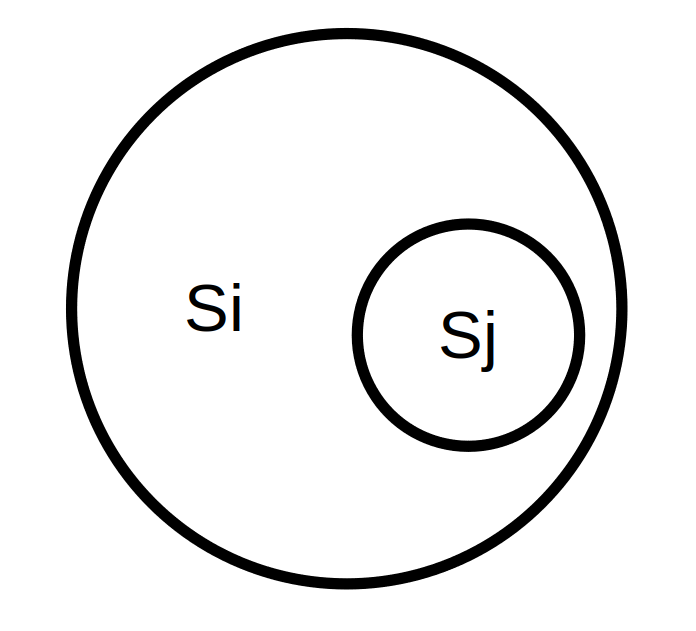
\includegraphics[scale=0.5]{images/fig_example.png}
	\label{fig:example}
\end{figure}

Рисунок \textit{\nameref{fig:example_scg}} показывает, как надо оформлять рисунки в SCg-коде. Параметр scale должен быть выставлен равным 0.8, для того чтобы все рисунки в SCg-коде имели одинаковый масштаб и размер идентификаторов примерно соответствовал размеру шрифта основного текста.  

\begin{figure}[H]
	\caption{SCg-текст. Пример рисунка в SCg-коде}
	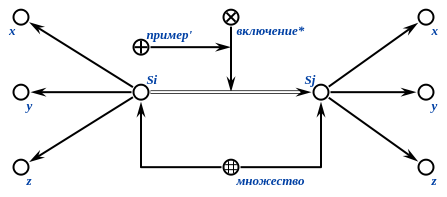
\includegraphics[scale=0.8]{images/fig_example_scg.png}
	\label{fig:example_scg}
\end{figure}
